\documentclass[11pt]{article}

% Usepackages 

\usepackage[utf8]{inputenc}
\usepackage[hmargin={1.5 cm,1.5cm},
   top=1.5cm, marginpar=3.5cm, bottom=1.5cm
   ]{geometry}  
\usepackage{subfiles}
\usepackage{hyperref}
\usepackage{physics}
\usepackage[most]{tcolorbox}
\usepackage{xparse}
\usepackage{accents}
\usepackage{pdfpages}
\usepackage{wrapfig}
\usepackage{amsmath}
\usepackage{amssymb}
\usepackage{amsthm}
\usepackage{amsfonts}
\usepackage{mathrsfs}
\usepackage{listings}
\usepackage{xcolor}
\usepackage{bbm}
\usepackage{tikz-cd}
\usepackage{tikz}
\usepackage{mathtools}
\usepackage{titlesec}
\usepackage[backend=biber, style=alphabetic, sorting=ynt]{biblatex}
%%%%%%%%

%Bibliography

%\addbibresource{ref.bib}

%%%%%%%%%

% Additional Styles

\hypersetup{colorlinks = true, linkcolor = blue, urlcolor = violet}

%\titleformat{\chapter}[display]{\normalfont\sffamily\Large\bfseries\centering}{\chaptertitlename\ \thechapter}{0pt}{\Huge}

\titleformat{\section}[hang]{\fontsize{14}{15}\sffamily\bfseries\centering}{\color{columbiablue}\S}{0.21em}{}

\newcommand{\textscf}[1]{\textbf{\textsc{#1}}}
%%%%%%
\definecolor{deepjunglegreen}{rgb}{0.40, 0.69, 0.29}
\definecolor{columbiablue}{rgb}{0.41, 0.37, .84}
%Theorem Box

\newtcbtheorem[no counter]{Thm}{\textbf{Theorem}}{
  breakable, enhanced,
  attach boxed title to top left={xshift=3mm, yshift=-3mm, yshifttext=-1mm},
  fonttitle=\sffamily,
  coltitle=blue!70,
  colbacktitle=white,
  %colbacktitle=cosmiclatte,
  colback=cyan!6,
  colframe=black!70,
  leftrule=0.5mm,
  rightrule=0.2mm,
  toprule=0.2mm,
  bottomrule=0.2mm,
  separator sign none, description delimiters parenthesis,
  description font=\mdseries}{th}

% defination Box

\newtcbtheorem[number within=section]{Def}{Definition}{
  breakable, enhanced,
  attach boxed title to top left={xshift=3mm, yshift=-3mm, yshifttext=-1mm},
  coltitle=black,
  colbacktitle=columbiablue!25,
  fonttitle=\sffamily,
  colback=white,
  colframe=black,
  leftrule=0.5mm,
  rightrule=0.2mm,
  toprule=0.2mm,
  bottomrule=0.2mm,
  arc=2.5mm,
  separator sign={\ $\blacktriangleright$},
  description delimiters none,
  description font=\bfseries}{def}

%Lemma
\definecolor{electricviolet}{rgb}{0.56, 0.0, 1.0}

\newtcbtheorem[no counter]{Lem}{ \textbf{\textcolor{electricviolet}{\S} Lemma:}}{
  detach title,
  fonttitle=\sffamily,
  coltitle=black,
  colbacktitle=white,
  colback=white,
  colframe=white,
  description font=\bfseries,
  before upper={\tcbtitle},
  title = $\mathbf{\S}$ \textsc{Lemma}
}{}

\newtcbtheorem[number within=section]{Lemn}{ \textbf{\textcolor{deepjunglegreen}{\S} Lemma}}{
  detach title,
  fonttitle=\sffamily,
  coltitle=black,
  colbacktitle=white,
  colback=white,
  colframe=white,
  description font=\bfseries,
  before upper={\tcbtitle},
  title = $\mathbf{\S}$ \textsc{Lemma}
}{}

%%% Info box 
\definecolor{corn}{rgb}{0.98, 0.93, 0.36}
\definecolor{awesome}{rgb}{1.0, 0.13, 0.32}
\definecolor{verdigris}{rgb}{0.26, 0.7, 0.68}
\definecolor{ufogreen}{rgb}{0.24, 0.82, 0.44}
\definecolor{turquoiseblue}{rgb}{0.0, 1.0, 0.94}
\definecolor{salmonpink}{rgb}{1.0, 0.57, 0.64}
\definecolor{screamin}{rgb}{0.46, 1.0, 0.44}
\newtcbtheorem[no counter]{Sly}{}{
 breakable, enhanced,
%   attach boxed title to top left={xshift=3mm, yshift= -3mm, yshifttext=-1mm},
  %coltitle=black,
  %colbacktitle=cyan!70,
  fonttitle=\sffamily,
  colback=cyan!5,
  colframe=black,
  leftrule=0.2mm,
  rightrule=0.2mm,
  toprule=0.2mm,
  bottomrule=0.2mm,
  separator sign none,
  description font=\bfseries}{}

%%%%%


%%%%problems
\definecolor{bondiblue}{rgb}{0.0, 0.58, 0.71}

\newtcbtheorem[no counter]{prob}{\textcolor{bondiblue}{\textbf{\textsf{Problem.}}}}{
  detach title,
  fonttitle=\sffamily,
  coltitle=black,
  colbacktitle=white,
  colback=white,
  colframe=white,
  leftrule=0.1mm,
  rightrule= -0.1mm,
  toprule=-0.1mm,
  bottomrule=-0.1mm,
  description font=\bfseries,
  before upper={\tcbtitle},
  title = $\mathbf{\S}$ 
}{}




% Main documentclass

\newcommand{\bb}[1]{\mathbb{#1}}
\newcommand{\N}{\bb{N}}
\newcommand{\Z}{\bb{Z}}
\newcommand{\Q}{\bb{Q}}
\newcommand{\R}{\mathbb{R}}
\newcommand{\C}{\bb{C}}
\newcommand{\Op}[1]{\mathcal{O}_{#1}}
\newcommand{\msk}{\medskip}
\newcommand{\ssk}{\smallskip}
\newcommand{\bsk}{\bigskip}
\newcommand{\Qed}{\quad \blacksquare}
\newcommand{\contra}{\rightarrow \leftarrow}
\newcommand{\heart}{\ensuremath\heartsuit}
\newcommand{\butt}{\rotatebox[origin=c]{180}{\heart}}
\newcommand{\ltag}[2]{\label{#1} \tag{#2}}
\newcommand{\floor}[1]{\lfloor {#1} \rfloor}
\newcommand{\inp}[2]{\left\langle {#1}, {#2} \right\rangle}
\newcommand{\vphi}{\varphi}
\newcommand{\veps}{\varepsilon}
\newcommand{\pdot}[2]{{#1} \cdot {#2}}
\newcommand{\Area}{\operatorname{Area}}
\newcommand{\ran}{\operatorname{ran}}
\newcommand{\Vol}{\operatorname{Vol}} 
\newcommand{\s}{\bb{S}}
\newcommand{\fb}[1]{\mathbf{#1}}
\newcommand{\T}{\mathbf{Top}}
\newcommand{\p}{\partial}
\newcommand{\ch}{\mathbf{Chain}^*}
\newcommand{\cha}{\mathbf{Chain}^\text{ag}}
\newcommand{\gr}{\mathbf{Graded groups}}
\newcommand{\kc}{\mathcal{K}}
\newcommand{\D}{\Delta}
\newcommand{\de}{\delta}
\newcommand{\ep}{\varepsilon}
\newcommand{\coro}[1]{{\hspace*{0.6cm} \textcolor{purple}{\textsc{Corollary. }}}\textit{#1}}
\newcommand{\examp}{\hspace{0.6cm} $\blacklozenge$ \textsc{Example} \textbf{:}} 
\newcommand{\ts}[1]{\textbf{\textsf{#1}}}
\newcommand{\cod}[1]{\textcolor{codegreen}{\texttt{#1}}}
\newcommand{\F}{\mathbb{F}}
\newcommand{\theo}[2]{{\hspace*{0.6cm} \textcolor{blue}{\textsc{Theorem.}}\hspace*{0.1cm}\textbf{\textsf{#1}} \hspace*{0.1cm}}\textit{#2}}
\newcommand{\sol}{ \textbf{\textit{Solution.}} }
\newcommand{\id}{\mathrm{id}}
%%%%%% 

\definecolor{codegreen}{rgb}{0,0.6,0}
\definecolor{codegray}{rgb}{0.5,0.5,0.5}
\definecolor{codepurple}{rgb}{0.58,0,0.82}
\definecolor{backcolour}{rgb}{1,1,1}

\lstdefinestyle{mystyle}{
    backgroundcolor=\color{backcolour},   
    commentstyle=\color{blue},
    keywordstyle=\color{magenta},
    numberstyle=\tiny\color{codegray},
    stringstyle=\color{codepurple},
    basicstyle=\ttfamily\footnotesize,
    breakatwhitespace=false,         
    breaklines=true,                 
    captionpos=b,                    
    keepspaces=true,                 
    numbers=left,                    
    numbersep=5pt,                  
    showspaces=false,                
    showstringspaces=false,
    showtabs=false,                  
    tabsize=2
}

\lstset{style=mystyle}


%%%%%%%

\begin{document}
 
 \title{{\Huge \textsc{Assignment-2}}}
 \author{\textbf{ \textsf{Algebraic Topology}} \\[0.2cm]
 \large \textsc{Trishan Mondal}}
 \date{}
 \maketitle

 ---------------------------------------------------------------------------------------------------------------------------------------------

 \section{Problem 1}

 \begin{prob}{}{}
    The goal of this exercise is to prove that the homotopy groups $\pi_n$ are abelian for $n \geq 2$. 
\begin{enumerate}
    \item[(a)] Let $S$ be a set equipped with two binary operations $\ast$ and $\circ$. Suppose that they have a common neutral element $e \in S$ and satisfy the interchange law 
    \[
        (a \ast b) \circ (c \ast d) = (a \circ c) \ast (b \circ d).    
    \] 
    Show that $\ast = \circ$ and that $a \ast b = b \ast a$. This is called the Eckmann-Hilton argument. 
    \item[(b)] Let $(X,x_0)$ be a pointed topological space and $\mu : X \times X \to X$ a pointed map such that $\mu(x_0, -) \simeq_* \id_X \simeq_* \mu(-,x_0)$. Show that the group $\pi_1(X,x_0)$ is abelian. 
    \item[(c)] Recall that $\pi_n(X,x_0)$ is the set of pointed homotopy classes of maps $I_n/\partial I_n \to (X,x_0)$. For each $1 \leq i \leq n$, there is a group operation $\ast_i$ on $\pi_n(X,x_0)$ induced by concatenating the $i$th direction: 
    \[
        \alpha \ast_i \beta (s_1,\dots,s_n) = \begin{cases}
            \alpha(s_1,\dots,2s_i, \dots, s_n) & \mbox{ if } s_i \in [0,1/2] \\ 
            \beta(s_1,\dots,2s_i - 1, \dots, s_n) & \mbox{ if } s_i \in [1/2,1].
        \end{cases}    
    \]
    If $n \geq 2$, show that all these group operations on $\pi_n(X,x_0)$ coincide and are abelian.
\end{enumerate}
 \end{prob}

 \sol Homotopy groups, $\pi_n$ are abelian for $n \geq 2$ is proved in the following steps which are solution to the consequent questions.

 \begin{itemize}
    \item[(a)] Both binary operation $\ast$ and $\circ$ has same neutral element. Call it $e$. Take $b = e$ and $c=e$ to get the following, 
    \begin{align*}
        (a \ast e) \circ (e \ast d) &= (a \circ e) \ast (e \circ d) \\
        \Rightarrow a \circ d &= a \ast d
    \end{align*}
    Since $a,d$ are aribitrary element of $S$ the operations $\ast$ and $\circ$ are same. Now take, $a = e$ and $d =e$ to get,
    \begin{align*}
        (e \ast b) \circ (c \ast e) &= (e \circ c) \ast (b \circ e) \\
        \Rightarrow b \circ c &= c \ast b\\
        \Rightarrow b\ast c &= c \ast b
    \end{align*}
    Here also $b$ and $c$ are aribitrary elements of $S$, we can say $a \ast b = b \ast a$ for all $a,b \in S$.
    \item[(b)] We will define an operation $\circ$ on $\pi_1(X,x_0)$. Let, $[\gamma], [\eta]$ are two elements of the fundamental group, define $[\gamma] \circ [\eta] = [\mu(\gamma,\eta)]$. Let, $\ast$ be the common product defined on $\pi_1 (X,x_0)$, which concatenates two loops in $X$. At the first hand we will show $\ast$ and $\circ$ has same neutral (identity) elements. We know $[c_{x_0}]$, the homotopy class of the constant map to $x_0$ is identity in $\pi_1(X,x_0)$. From the given condition we can say, $$[c_{x_0}]\circ [\gamma]=[\mu(c_{x_0}, \gamma)] = [\gamma] = \mu[(\gamma,c_{x_0})]=[\gamma]\circ [c_{x_0}]$$
    The second and third equality follows from the fact $\mu(x_0, -) \simeq_* \id_X \simeq_* \mu(-,x_0)$. Let, $[f],[g],[h],[k]$ are four elements of $\pi_1(X,x_0)$, 
    \begin{align*}
       \mu (f\ast g, h\ast k) &= \begin{cases}
        \mu(f(2t),h(2t)) & \text{ if } t\in [0,\frac{1}{2}] \\
        \mu (g(2t-1),k(2t-1)) & \text{ if } t \in [\frac{1}{2},1]
       \end{cases} \\
       &= \mu(f,h) \ast \mu(g,k)
    \end{align*}
    Thus we have $([f]\ast[g])\circ([h]\ast [k]) = ([f]\circ [h])\ast ([g]\circ [k])$. From the previous part we can say $\ast$ and $\circ$ defines same operation on $\pi_1(X,x_0)$ and they are abelian and hence $\pi_1(X,x_0)$ is abelian. 
    \item[(c)] Notice that, $\ast_i$ is a group operation. This can be shown in the same way we have proved concatenation of loops gives a group operation in Fundamental group. We will begin with showing, $([f] \ast_1 [g])\ast_2([h] \ast_1 [k])=([f]\ast_2[h]) \ast_1 ([g]\ast_2[k])$ and then we will show that $\ast_1$ and $\ast_2$ has same neutral element. Then by part (a) we can conclude $\ast_1 = \ast_2$ and $\pi_n(X,x_0)$ is abelian. The left-hand side is defined to be the homotopy class of

    $$
    (f \ast_1  g)\ast_2(h \ast_1  k)\left(t_{1}, \ldots, t_{n}\right)= \begin{cases}f\left(2 t_{1}, 2 t_{2}, t_{3} \ldots, t_{n}\right) & t_{1} \leq 1 / 2, t_{2} \leq 1 / 2 \\ g\left(2 t_{1}, 2 t_{2}-1, t_{3}, \ldots, t_{n}\right) & t_{1} \leq 1 / 2, t_{2} \geq 1 / 2 \\ h\left(2 t_{1}-1,2 t_{2}, t_{3} \ldots, t_{n}\right) & t_{1} \geq 1 / 2, t_{2} \leq 1 / 2 \\ k\left(2 t_{1}-1,2 t_{2}-1, t_{3}, \ldots, t_{n}\right) & t_{1} \geq 1 / 2, t_{2} \geq 1 / 2 .\end{cases}
    $$
    The right hand side is the homotopy class of

$$
(f\ast_2 h) \ast_1 (g\ast_2 k)\left(t_{1}, \ldots, t_{n}\right)= \begin{cases}f\left(2 t_{1}, 2 t_{2}, t_{3} \ldots, t_{n}\right) & t_{1} \leq 1 / 2, t_{2} \leq 1 / 2 \\ h\left(2 t_{1}-1,2 t_{2}, t_{3} \ldots, t_{n}\right) & t_{1} \geq 1 / 2, t_{2} \leq 1 / 2 \\ g\left(2 t_{1}, 2 t_{2}-1, t_{3}, \ldots, t_{n}\right) & t_{1} \leq 1 / 2, t_{2} \geq 1 / 2 \\ k\left(2 t_{1}-1,2 t_{2}-1, t_{3}, \ldots, t_{n}\right) & t_{1} \geq 1 / 2, t_{2} \geq 1 / 2 .\end{cases}
$$
    Thus we have shown $([f] \ast_1 [g])\ast_2([h] \ast_1 [k])=([f]\ast_2[h]) \ast_1 ([g]\ast_2[k])$. Let, $c_{x_0}$ be the constant map $c_{x_0}:(I^n,\p I^n) \to (X,x_0)$. Note that,
     \begin{align*}
        f\ast_1  c_{x_0} &= \begin{cases}
            f(2t_1,t_2,\cdots,t_n) & t_1 \leq \frac{1}{2}\\
            c_{x_0} & t_1 \geq \frac{1}{2}
        \end{cases} \\
        f\ast_2  c_{x_0} &= \begin{cases}
            f(t_1,2t_2,\cdots,t_n) & t_2 \leq \frac{1}{2}\\
            c_{x_0} & t_2 \geq \frac{1}{2}
        \end{cases} 
    \end{align*}
    We can show, $[f\ast_1  c_{x_0}]=[f]$ and $[f\ast_2  c_{x_0}] = [f]$, in the same way we proved constant map is identity for the fundamental group. Thus both $\ast_1$ and $\ast_2$ has same neutral element. Thus $\ast_1$ and $\ast_2$ are same operation. In the same way we can prove $\ast_i$ and $\ast_j$ are same operation for $i \neq j$. And hence $\pi_n(X,x_0)$ is abelian. $\hfill \blacksquare$
 \end{itemize}
 

\section{Problem2}

 \begin{prob}{}{}
    Every closed connected surface is homeomorphic to $\Sigma_g$ for some some $g \geq 0$ or to $N_h$ for some $h \geq 1$, where $\Sigma_g$ (respectively $N_h$) is obtained from a sphere by attaching $g$ copies of the torus $\s^1 \times \s^1$. (respectively $h$ copies of the real projective plane $\R P^2$). For each of the following surfaces, give a presentation of the fundamental group and compute its abelianization as a direct sum of groups of the form $\Z/n\Z$ (recall that the abelianization of a group $G$ is the abelian group $G^{ab} = G/[G,G]$). 
\begin{enumerate}
    \item[(a)] The genus $2$ surfaces $\Sigma_2$. 
    \item[(b)] The Klein bottle $N_2$. 
    \item[(c)] The remaining closed surfaces $\Sigma_g$ and $N_h$ for $g,h \geq 3$.   
\end{enumerate}
 \end{prob}

 \sol We will try to derive the presentation of fundamental group for $\Sigma_g$ and $N_g$, as a corollary to that we will give the presentation of $\Sigma_2$ and $N_2$. We will start with proving the following lemmas regarding polygonal presentation of the surfaces $\Sigma_g$ and $N_g$. 

 \begin{Lemn}{ }{}
    The space \( \Sigma_g \) has the polygonal presentation given by a \( 4g- \)gon, with sides labelled as \( a_1,b_1,a_1^{-1}, b_1^{-1}, \dots, a_g,b_g,a_g^{-1}, b_g^{-1} \). 
 \end{Lemn}\label{lem:1}

 \noindent \textit{Proof.} We prove this statement using mathematical induction on the variable \( g \). Initially, we establish the base case for \( g = 1 \) based on the standard definition of the torus. For the induction step, we assume the statement holds true for some \( g \geq 1 \). Now, let's consider the pus-out square that generates \( \Sigma_{g+1} \) from \( \Sigma_g \), depicted below:
  
 \[\begin{tikzcd}
    {\p D^2} && T\setminus D^2 \\
    \\
    {\Sigma_g\setminus D^2} && {\Sigma_{g+1}}
    \arrow[hook, from=1-1, to=1-3]
    \arrow[hook', from=1-1, to=3-1]
    \arrow[from=3-1, to=3-3]
    \arrow[from=1-3, to=3-3]
  \end{tikzcd}\]
 When we remove a disk from \( \Sigma_g \), and torus $T$, then adjoin them along their boundary we will get $\Sigma_{g+1}$. This process is equivalent to adding an edge to the polygonal representation. Notably, this new edge becomes identified with the edge added to the polygonal representation of \( T \). As a result, the polygonal presentation of \( \Sigma_{g+1} \) consists of a \( 4(g+1) \)-gon with sides labeled as follows:
 
 \[  a_1, b_1, a_1^{-1}, b_1^{-1}, \dots, a_g, b_g, a_g^{-1}, b_g^{-1}, a, b, a^{-1}, b^{-1} \]
 Consequently, we can conclude that the statement holds true for all \( g \geq 1 \) by induction.
 
 \begin{figure}[htbp]
      \centering
      \tikzset{every picture/.style={line width=0.75pt}} %set default line width to 0.75pt        

      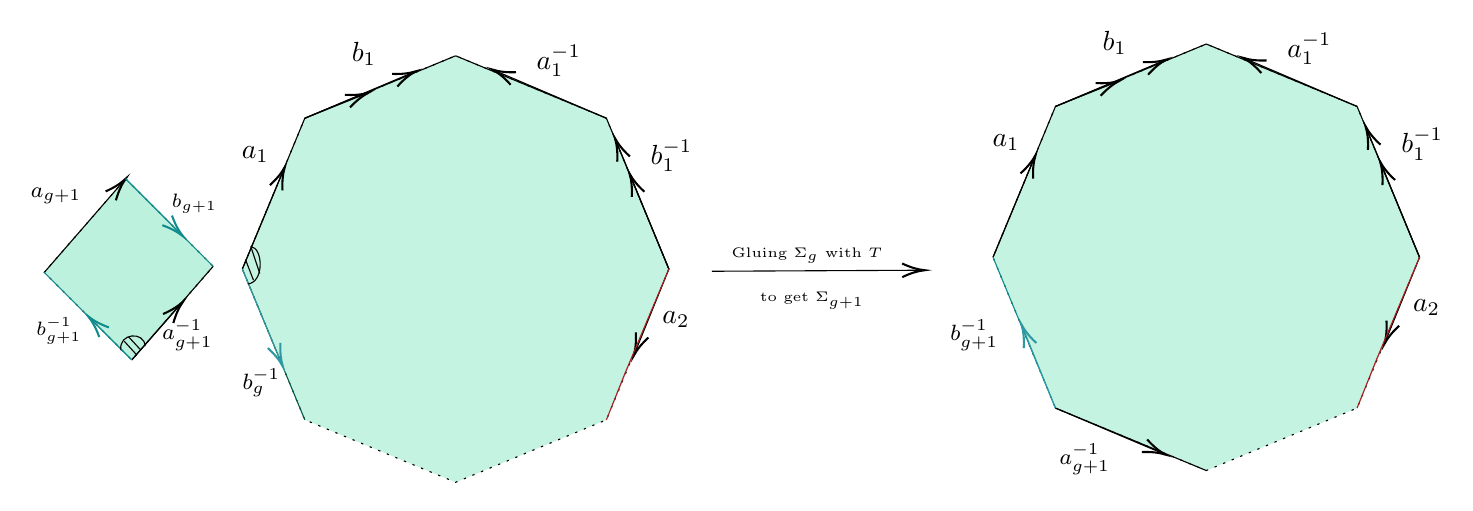
\begin{tikzpicture}[x=0.75pt,y=0.75pt,yscale=-1,xscale=1]
      %uncomment if require: \path (0,268); %set diagram left start at 0, and has height of 268
      
      %Shape: Regular Polygon [id:dp5141607886215573] 
      \draw  [fill={rgb, 255:red, 188; green, 241; blue, 222 }  ,fill opacity=0.88 ][dash pattern={on 0.84pt off 2.51pt}] (321.33,139.42) -- (291.24,212.07) -- (218.58,242.17) -- (145.93,212.07) -- (115.83,139.42) -- (145.93,66.76) -- (218.58,36.67) -- (291.24,66.76) -- cycle ;
      %Straight Lines [id:da5153171721627441] 
      \draw    (115.83,139.42) -- (127.85,110.55) -- (135.56,92.01) ;
      \draw [shift={(136.33,90.17)}, rotate = 112.6] [color={rgb, 255:red, 0; green, 0; blue, 0 }  ][line width=0.75]    (10.93,-3.29) .. controls (6.95,-1.4) and (3.31,-0.3) .. (0,0) .. controls (3.31,0.3) and (6.95,1.4) .. (10.93,3.29)   ;
      %Straight Lines [id:da5037769564001415] 
      \draw    (145.93,66.76) -- (197.49,44.95) ;
      \draw [shift={(199.33,44.17)}, rotate = 157.07] [color={rgb, 255:red, 0; green, 0; blue, 0 }  ][line width=0.75]    (10.93,-3.29) .. controls (6.95,-1.4) and (3.31,-0.3) .. (0,0) .. controls (3.31,0.3) and (6.95,1.4) .. (10.93,3.29)   ;
      %Straight Lines [id:da1602860790882703] 
      \draw    (145.93,66.76) -- (174.77,55.21) ;
      \draw [shift={(176.63,54.46)}, rotate = 158.17] [color={rgb, 255:red, 0; green, 0; blue, 0 }  ][line width=0.75]    (10.93,-3.29) .. controls (6.95,-1.4) and (3.31,-0.3) .. (0,0) .. controls (3.31,0.3) and (6.95,1.4) .. (10.93,3.29)   ;
      %Straight Lines [id:da45327565311835794] 
      \draw    (291.24,66.76) -- (238.17,44.11) ;
      \draw [shift={(236.33,43.32)}, rotate = 23.12] [color={rgb, 255:red, 0; green, 0; blue, 0 }  ][line width=0.75]    (10.93,-3.29) .. controls (6.95,-1.4) and (3.31,-0.3) .. (0,0) .. controls (3.31,0.3) and (6.95,1.4) .. (10.93,3.29)   ;
      %Straight Lines [id:da5102257748117363] 
      \draw    (321.33,139.42) -- (296.1,78.17) ;
      \draw [shift={(295.33,76.32)}, rotate = 67.6] [color={rgb, 255:red, 0; green, 0; blue, 0 }  ][line width=0.75]    (10.93,-3.29) .. controls (6.95,-1.4) and (3.31,-0.3) .. (0,0) .. controls (3.31,0.3) and (6.95,1.4) .. (10.93,3.29)   ;
      %Straight Lines [id:da4541147110427879] 
      \draw    (321.33,139.42) -- (303.1,95.17) ;
      \draw [shift={(302.33,93.32)}, rotate = 67.6] [color={rgb, 255:red, 0; green, 0; blue, 0 }  ][line width=0.75]    (10.93,-3.29) .. controls (6.95,-1.4) and (3.31,-0.3) .. (0,0) .. controls (3.31,0.3) and (6.95,1.4) .. (10.93,3.29)   ;
      %Straight Lines [id:da8741026059338475] 
      \draw [draw opacity=0][fill={rgb, 255:red, 208; green, 2; blue, 27 }  ,fill opacity=1 ]   (321.33,139.42) -- (292,210.22) ;
      \draw [shift={(291.24,212.07)}, rotate = 292.5] [draw opacity=0][line width=0.75]    (10.93,-3.29) .. controls (6.95,-1.4) and (3.31,-0.3) .. (0,0) .. controls (3.31,0.3) and (6.95,1.4) .. (10.93,3.29)   ;
      %Straight Lines [id:da49284860101511807] 
      \draw [fill={rgb, 255:red, 136; green, 19; blue, 19 }  ,fill opacity=1 ]   (321.33,139.42) -- (314.94,155.17) -- (305.09,179.47) ;
      \draw [shift={(304.33,181.32)}, rotate = 292.08] [color={rgb, 255:red, 0; green, 0; blue, 0 }  ][line width=0.75]    (10.93,-3.29) .. controls (6.95,-1.4) and (3.31,-0.3) .. (0,0) .. controls (3.31,0.3) and (6.95,1.4) .. (10.93,3.29)   ;
      %Straight Lines [id:da9725759711034252] 
      \draw    (115.83,139.42) -- (145.93,66.76) ;
      %Straight Lines [id:da5424103036641399] 
      \draw    (145.93,66.76) -- (218.58,36.67) ;
      %Straight Lines [id:da09045611747914295] 
      \draw    (218.58,36.67) -- (291.24,66.76) ;
      %Straight Lines [id:da8305451917048523] 
      \draw    (291.24,66.76) -- (321.33,139.42) ;
      %Straight Lines [id:da03736308423725454] 
      \draw [color={rgb, 255:red, 169; green, 32; blue, 32 }  ,draw opacity=1 ]   (321.33,139.42) -- (300.33,189.32) -- (291.24,212.07) ;
      %Straight Lines [id:da9974477846717058] 
      \draw [color={rgb, 255:red, 4; green, 92; blue, 72 }  ,draw opacity=1 ]   (115.83,139.42) -- (145.93,212.07) ;
      %Straight Lines [id:da36054738927648033] 
      \draw [color={rgb, 255:red, 46; green, 153; blue, 162 }  ,draw opacity=1 ]   (115.83,139.42) -- (134.57,184.48) ;
      \draw [shift={(135.33,186.32)}, rotate = 247.43] [color={rgb, 255:red, 46; green, 153; blue, 162 }  ,draw opacity=1 ][line width=0.75]    (10.93,-3.29) .. controls (6.95,-1.4) and (3.31,-0.3) .. (0,0) .. controls (3.31,0.3) and (6.95,1.4) .. (10.93,3.29)   ;
      %Curve Lines [id:da26706500081736695] 
      \draw    (119.89,128.55) .. controls (125.89,129.21) and (126.44,145.94) .. (118.44,146.6) ;
      %Straight Lines [id:da38812411755326237] 
      \draw    (117.33,134.82) -- (121.17,144.74) ;
      %Straight Lines [id:da3452144988874781] 
      \draw    (119.89,128.55) -- (124.22,141.49) ;
      %Shape: Square [id:dp8672460876012633] 
      \draw  [fill={rgb, 255:red, 188; green, 241; blue, 222 }  ,fill opacity=1 ][dash pattern={on 0.84pt off 2.51pt}] (59.61,95.92) -- (101.79,138.1) -- (62.56,183.22) -- (20.39,141.05) -- cycle ;
      %Straight Lines [id:da3394864684004628] 
      \draw    (20.39,141.05) -- (58.3,97.43) ;
      \draw [shift={(59.61,95.92)}, rotate = 131] [color={rgb, 255:red, 0; green, 0; blue, 0 }  ][line width=0.75]    (10.93,-3.29) .. controls (6.95,-1.4) and (3.31,-0.3) .. (0,0) .. controls (3.31,0.3) and (6.95,1.4) .. (10.93,3.29)   ;
      %Straight Lines [id:da3604010000185156] 
      \draw [color={rgb, 255:red, 17; green, 139; blue, 141 }  ,draw opacity=1 ]   (59.61,95.92) -- (101.79,138.1) ;
      %Straight Lines [id:da7237873302090645] 
      \draw    (62.56,183.22) -- (101.79,138.1) ;
      %Straight Lines [id:da4470449700914103] 
      \draw [color={rgb, 255:red, 17; green, 139; blue, 141 }  ,draw opacity=1 ]   (20.39,141.05) -- (62.56,183.22) ;
      %Straight Lines [id:da23184927370680697] 
      \draw [color={rgb, 255:red, 17; green, 139; blue, 141 }  ,draw opacity=1 ]   (59.61,95.92) -- (85.92,122.3) ;
      \draw [shift={(87.33,123.72)}, rotate = 225.07] [color={rgb, 255:red, 17; green, 139; blue, 141 }  ,draw opacity=1 ][line width=0.75]    (10.93,-3.29) .. controls (6.95,-1.4) and (3.31,-0.3) .. (0,0) .. controls (3.31,0.3) and (6.95,1.4) .. (10.93,3.29)   ;
      %Straight Lines [id:da6338478011519619] 
      \draw    (62.56,183.22) -- (86.01,156.55) ;
      \draw [shift={(87.33,155.05)}, rotate = 131.33] [color={rgb, 255:red, 0; green, 0; blue, 0 }  ][line width=0.75]    (10.93,-3.29) .. controls (6.95,-1.4) and (3.31,-0.3) .. (0,0) .. controls (3.31,0.3) and (6.95,1.4) .. (10.93,3.29)   ;
      %Straight Lines [id:da0851986405075531] 
      \draw [color={rgb, 255:red, 17; green, 139; blue, 141 }  ,draw opacity=1 ]   (62.56,183.22) -- (42.89,163.55) ;
      \draw [shift={(41.48,162.13)}, rotate = 45] [color={rgb, 255:red, 17; green, 139; blue, 141 }  ,draw opacity=1 ][line width=0.75]    (10.93,-3.29) .. controls (6.95,-1.4) and (3.31,-0.3) .. (0,0) .. controls (3.31,0.3) and (6.95,1.4) .. (10.93,3.29)   ;
      %Shape: Regular Polygon [id:dp41014614704630903] 
      \draw  [fill={rgb, 255:red, 188; green, 241; blue, 222 }  ,fill opacity=0.88 ][dash pattern={on 0.84pt off 2.51pt}] (683,133.75) -- (652.91,206.41) -- (580.25,236.5) -- (507.59,206.41) -- (477.5,133.75) -- (507.59,61.09) -- (580.25,31) -- (652.91,61.09) -- cycle ;
      %Straight Lines [id:da5179448077631912] 
      \draw    (477.5,133.75) -- (489.52,104.88) -- (497.23,86.35) ;
      \draw [shift={(498,84.5)}, rotate = 112.6] [color={rgb, 255:red, 0; green, 0; blue, 0 }  ][line width=0.75]    (10.93,-3.29) .. controls (6.95,-1.4) and (3.31,-0.3) .. (0,0) .. controls (3.31,0.3) and (6.95,1.4) .. (10.93,3.29)   ;
      %Straight Lines [id:da14683792457808598] 
      \draw    (507.59,61.09) -- (559.16,39.28) ;
      \draw [shift={(561,38.5)}, rotate = 157.07] [color={rgb, 255:red, 0; green, 0; blue, 0 }  ][line width=0.75]    (10.93,-3.29) .. controls (6.95,-1.4) and (3.31,-0.3) .. (0,0) .. controls (3.31,0.3) and (6.95,1.4) .. (10.93,3.29)   ;
      %Straight Lines [id:da6367837200145838] 
      \draw    (507.59,61.09) -- (536.44,49.54) ;
      \draw [shift={(538.3,48.8)}, rotate = 158.17] [color={rgb, 255:red, 0; green, 0; blue, 0 }  ][line width=0.75]    (10.93,-3.29) .. controls (6.95,-1.4) and (3.31,-0.3) .. (0,0) .. controls (3.31,0.3) and (6.95,1.4) .. (10.93,3.29)   ;
      %Straight Lines [id:da023146452148977925] 
      \draw    (652.91,61.09) -- (599.84,38.44) ;
      \draw [shift={(598,37.66)}, rotate = 23.12] [color={rgb, 255:red, 0; green, 0; blue, 0 }  ][line width=0.75]    (10.93,-3.29) .. controls (6.95,-1.4) and (3.31,-0.3) .. (0,0) .. controls (3.31,0.3) and (6.95,1.4) .. (10.93,3.29)   ;
      %Straight Lines [id:da19305069349361292] 
      \draw    (683,133.75) -- (657.76,72.51) ;
      \draw [shift={(657,70.66)}, rotate = 67.6] [color={rgb, 255:red, 0; green, 0; blue, 0 }  ][line width=0.75]    (10.93,-3.29) .. controls (6.95,-1.4) and (3.31,-0.3) .. (0,0) .. controls (3.31,0.3) and (6.95,1.4) .. (10.93,3.29)   ;
      %Straight Lines [id:da7752407728423769] 
      \draw    (683,133.75) -- (664.76,89.51) ;
      \draw [shift={(664,87.66)}, rotate = 67.6] [color={rgb, 255:red, 0; green, 0; blue, 0 }  ][line width=0.75]    (10.93,-3.29) .. controls (6.95,-1.4) and (3.31,-0.3) .. (0,0) .. controls (3.31,0.3) and (6.95,1.4) .. (10.93,3.29)   ;
      %Straight Lines [id:da28145489053166295] 
      \draw [draw opacity=0][fill={rgb, 255:red, 208; green, 2; blue, 27 }  ,fill opacity=1 ]   (683,133.75) -- (653.67,204.56) ;
      \draw [shift={(652.91,206.41)}, rotate = 292.5] [draw opacity=0][line width=0.75]    (10.93,-3.29) .. controls (6.95,-1.4) and (3.31,-0.3) .. (0,0) .. controls (3.31,0.3) and (6.95,1.4) .. (10.93,3.29)   ;
      %Straight Lines [id:da8123191900360864] 
      \draw [fill={rgb, 255:red, 136; green, 19; blue, 19 }  ,fill opacity=1 ]   (683,133.75) -- (676.61,149.5) -- (666.75,173.8) ;
      \draw [shift={(666,175.66)}, rotate = 292.08] [color={rgb, 255:red, 0; green, 0; blue, 0 }  ][line width=0.75]    (10.93,-3.29) .. controls (6.95,-1.4) and (3.31,-0.3) .. (0,0) .. controls (3.31,0.3) and (6.95,1.4) .. (10.93,3.29)   ;
      %Straight Lines [id:da1263446396353023] 
      \draw    (477.5,133.75) -- (507.59,61.09) ;
      %Straight Lines [id:da48020167148605153] 
      \draw    (507.59,61.09) -- (580.25,31) ;
      %Straight Lines [id:da06904867808658599] 
      \draw    (580.25,31) -- (652.91,61.09) ;
      %Straight Lines [id:da7677586897201767] 
      \draw    (652.91,61.09) -- (683,133.75) ;
      %Straight Lines [id:da20676241898208514] 
      \draw [color={rgb, 255:red, 169; green, 32; blue, 32 }  ,draw opacity=1 ]   (683,133.75) -- (662,183.66) -- (652.91,206.41) ;
      %Straight Lines [id:da1925111716512129] 
      \draw [color={rgb, 255:red, 17; green, 139; blue, 141 }  ,draw opacity=1 ]   (477.5,133.75) -- (507.59,206.41) ;
      %Straight Lines [id:da7719683350182798] 
      \draw [color={rgb, 255:red, 46; green, 153; blue, 162 }  ,draw opacity=1 ]   (507.59,206.41) -- (491.98,168.01) ;
      \draw [shift={(491.22,166.16)}, rotate = 67.86] [color={rgb, 255:red, 46; green, 153; blue, 162 }  ,draw opacity=1 ][line width=0.75]    (10.93,-3.29) .. controls (6.95,-1.4) and (3.31,-0.3) .. (0,0) .. controls (3.31,0.3) and (6.95,1.4) .. (10.93,3.29)   ;
      %Curve Lines [id:da5388414821915835] 
      \draw    (57.33,178.55) .. controls (56,170.21) and (68.67,169.21) .. (69,176.55) ;
      %Straight Lines [id:da6584805104260762] 
      \draw    (58.89,174.16) -- (65,180.88) ;
      %Straight Lines [id:da6680002917140142] 
      \draw    (61,172.05) -- (67,178.55) ;
      %Straight Lines [id:da7168960800797919] 
      \draw    (507.59,206.41) -- (580.25,236.5) ;
      %Straight Lines [id:da3005485698539254] 
      \draw    (507.59,206.41) -- (558.71,228.05) ;
      \draw [shift={(560.56,228.83)}, rotate = 202.95] [color={rgb, 255:red, 0; green, 0; blue, 0 }  ][line width=0.75]    (10.93,-3.29) .. controls (6.95,-1.4) and (3.31,-0.3) .. (0,0) .. controls (3.31,0.3) and (6.95,1.4) .. (10.93,3.29)   ;
      %Straight Lines [id:da36792994846117444] 
      \draw    (342,140.49) -- (442.67,140) ;
      \draw [shift={(444.67,139.99)}, rotate = 179.72] [color={rgb, 255:red, 0; green, 0; blue, 0 }  ][line width=0.75]    (10.93,-3.29) .. controls (6.95,-1.4) and (3.31,-0.3) .. (0,0) .. controls (3.31,0.3) and (6.95,1.4) .. (10.93,3.29)   ;

% Text Node
\draw (114.33,79.07) node [anchor=north west][inner sep=0.75pt]    {$a_{1}$};
% Text Node
\draw (167.33,29.07) node [anchor=north west][inner sep=0.75pt]    {$b_{1}$};
% Text Node
\draw (256.33,30.07) node [anchor=north west][inner sep=0.75pt]    {$a_{1}^{-1}$};
% Text Node
\draw (311.33,76.07) node [anchor=north west][inner sep=0.75pt]    {$b_{1}^{-1}$};
% Text Node
\draw (316.94,158.57) node [anchor=north west][inner sep=0.75pt]    {$a_{2}$};
% Text Node
\draw (114.67,186.4) node [anchor=north west][inner sep=0.75pt]  [font=\footnotesize]  {$b_{g}^{-1}$};
% Text Node
\draw (12.67,99.07) node [anchor=north west][inner sep=0.75pt]  [font=\footnotesize]  {$a_{g+1}$};
% Text Node
\draw (80.67,102.07) node [anchor=north west][inner sep=0.75pt]  [font=\scriptsize]  {$b_{g+1}$};
% Text Node
\draw (15.33,161.4) node [anchor=north west][inner sep=0.75pt]  [font=\scriptsize]  {$b_{g+1}^{-1}$};
% Text Node
\draw (76,162.4) node [anchor=north west][inner sep=0.75pt]  [font=\footnotesize]  {$a_{g+1}^{-1}$};
% Text Node
\draw (476,73.4) node [anchor=north west][inner sep=0.75pt]    {$a_{1}$};
% Text Node
\draw (529,23.4) node [anchor=north west][inner sep=0.75pt]    {$b_{1}$};
% Text Node
\draw (618,24.4) node [anchor=north west][inner sep=0.75pt]    {$a_{1}^{-1}$};
% Text Node
\draw (673,70.4) node [anchor=north west][inner sep=0.75pt]    {$b_{1}^{-1}$};
% Text Node
\draw (678.61,152.9) node [anchor=north west][inner sep=0.75pt]    {$a_{2}$};
% Text Node
\draw (455.67,162.73) node [anchor=north west][inner sep=0.75pt]  [font=\footnotesize]  {$b_{g+1}^{-1}$};
% Text Node
\draw (508.33,222.4) node [anchor=north west][inner sep=0.75pt]  [font=\footnotesize]  {$a_{g+1}^{-1}$};
% Text Node
\draw (350.33,128) node [anchor=north west][inner sep=0.75pt]  [font=\tiny]  {$\text{Gluing } \Sigma_g \text{ with } T$};
% Text Node
\draw (396.67,127.67) node [anchor=north west][inner sep=0.75pt]  [font=\tiny]  {};
% Text Node
\draw (406.67,170.27) node  [font=\tiny] [align=left] {\begin{minipage}[lt]{80.24pt}\setlength\topsep{0pt}

\end{minipage}};
% Text Node
\draw (364,149.34) node [anchor=north west][inner sep=0.75pt]  [font=\tiny]  {$\text{to get } \Sigma_{g+1}$};


     \end{tikzpicture}
\end{figure}


 \begin{Lemn}{ }{}
    The space \( N_h \) has the polygonal presentation given by a \( 2g- \)gon, with sides labelled as \( a_1, a_1, \dots, a_g, a_g \).
 \end{Lemn} \label{lem:2}

 \noindent \textit{Proof.}   The proof is essentially same as above and by the same arguments as above and the fact that \( N_1 \simeq \mathbb{R}P^2 \) has the polygonal presentation given by a \( 2- \)gon with sides labelled as \( a_1, a_1 \). $\hfill \blacksquare$




 \noindent Using the polygonal presentation in Lemma \ref{lem:1}.1, we get \( \Sigma_g \) is also a result of the following pushout, 
 \[\begin{tikzcd}
    \mathbb{S}^1 && \bigvee_{i=1}^{2g} \mathbb{S}^1 \\
    \\
    D^2 && {\Sigma_{g}}
    \arrow[hook, "\varphi", from=1-1, to=1-3]
    \arrow[hook', from=1-1, to=3-1]
    \arrow[from=3-1, to=3-3]
    \arrow[from=1-3, to=3-3]
  \end{tikzcd}\]
  where \( \varphi \) induces the word \( a_1b_1a_1^{-1}b_1^{-1} \cdots a_gb_ga_g^{-1}b_g^{-1} \), if \( a_1, b_1, \dots, a_g, b_g \) are the generators of the fundamental group \( \pi_1(\bigvee_{i=1}^{2g} \mathbb{S}^1) \). Hence, using the result of Problem 8 of Assignment 1 (attaching of cells), we get
  \[
    \pi_1(\Sigma_g) \simeq \pi_1\left(\bigvee_{i=1}^{2g} \mathbb{S}^1\right) \Bigg/ N \simeq \left\langle {a_1, b_1, \dots, a_g, b_g} \mid {[a_1,b_1]\cdots [a_g,b_g]} \right\rangle
  \]
Let's consider the commutator \([x, y] = xyx^{-1}y^{-1}\), where \(N\) represents the normal subgroup of \(\pi_1(\bigvee_{i=1}^{2g})\s^1\) generated by the elements \(\{[a_1, b_1], \ldots, [a_g, b_g]\}\). When we take the abelianization, we obtain \({\pi_1(\Sigma_g)}^{\text{ab}} \simeq \mathbb{Z}^{2g}\), because all commutators become trivial in an abelian group.
  
\noindent \textbf{Part(a)} In particular, for \(g = 2\), we have:
\begin{align*}
    &\pi_1(\Sigma_2) \simeq \left\langle {a_1, b_1, a_2, b_2} \mid {a_1b_1a_1^{-1}b_1^{-1}a_2b_2a_2^{-1}b_2^{-1}} \right\rangle\\
     &\implies {\pi_1(\Sigma_2)}^{\text{ab}} \simeq \mathbb{Z}^{4}
\end{align*}
Utilizing the polygonal representation as outlined in Lemma \ref{lem:2}.2, we can deduce that \( N_h \) also takes the form of the following pushout:

\[
\begin{tikzcd}
\mathbb{S}^1 && \bigvee_{i=1}^{h} \mathbb{S}^1 \\
\\
D^2 && {N_h}
\arrow[hook, "\psi", from=1-1, to=1-3]
\arrow[hook', from=1-1, to=3-1]
\arrow[from=3-1, to=3-3]
\arrow[from=1-3, to=3-3]
\end{tikzcd}
\]
Here, \( \psi \) induces the word \( a_1^2 \cdots a_h^2 \), provided that \( a_1, \dots, a_h \) represent the generators of the fundamental group \( \pi_1(\bigvee_{i=1}^{h} \mathbb{S}^1) \). Consequently, by leveraging the outcome of Problem 8 from Assignment 1 (pertaining to cell attachments), we obtain, 
\[
    \pi_1(N_h) \simeq \pi_1\left(\bigvee_{i=1}^{h} \mathbb{S}^1\right) \Bigg/ M \simeq \left\langle {a_1, \dots, a_h} \mid {a_1^2\cdots a_h^2} \right\rangle
\]
where \( M \) is the normal subgroup of \( \pi_1(\bigvee_{i=1}^{h}\mathbb{S}^1) \) generated by \( \{a_1^2\cdots a_h^2\} \). Taking the abelianization, we get \( {\pi_1(N_h)}^{\text{ab}} \simeq \mathbb{Z}^h/\left\langle 2(a_1+\cdots+a_h) = 0 \right\rangle \).

\vspace*{0.2cm}

\noindent \textbf{Part(b)} For \( h=2 \) we get
\[
  \pi_1(N_2) \simeq \left\langle a_1, a_2 \mid {a_1^2a_2^2} \right\rangle = \left\langle {a,b}\mid  {aba^{-1}b} \right\rangle
\]
where the last equality is obtained by putting \( a = a_1, b = a_1a_2 \). Taking the abelianization we get,
\[
  {\pi_1(N_2)}^{\text{ab}} \simeq \left\langle {a,b}\mid {b^2 = 1, ab =ba} \right\rangle \simeq \mathbb{Z} \times \mathbb{Z}/2 \mathbb{Z}
\]



 \section{Problem 3}

 \begin{prob}{}{}
    Describe upto isomorphism all path connected 2-sheeted covering spaces of:
\begin{enumerate}
    \item[(a)] the M\"{o}bius strip $\mu$
    \item[(b)] the torus $\s^1 \times \s^1$
    \item[(c)] the figure eight $\s^1 \vee \s^1$.   
\end{enumerate}
 \end{prob}
\sol
 \begin{itemize}
    \item[(a)]  Consider the action of $\Z$ on $X=\R \times [-1,1]$, defined by $n \cdot (x,y) \mapsto (x+n,(-1)^ny)$. This is well-defined action of $\Z$ on $X$. This action is properly discontinuous. For every point $(x,y)$ after action of $g\in \Z$ on it, $x$ co-ordinate is translated $\abs{g}$ distance, so the action is not free. Now take an open ball centered at $(x,y)$ of $\frac{1}{2}$ radius, call it $U$. Note that, $U \cup g.U =\emptyset$. So the action is properly discontinuous. The projection map $\pi : X \to X/\Z$ is a covering map. Since, $X$ is simply connected $\pi_1(X/\Z) =\Z$.  We will show this orbit-space is actually a Mobius strip. 
    
     \begin{figure}[htbp]
          \centering 
          \tikzset{every picture/.style={line width=0.75pt}} %set default line width to 0.75pt        

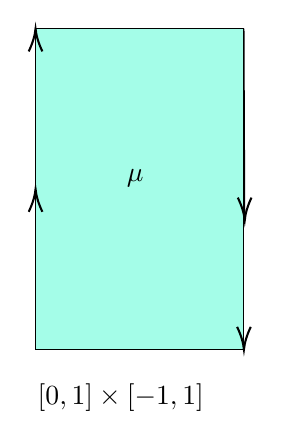
\begin{tikzpicture}[x=0.75pt,y=0.75pt,yscale=-1,xscale=1]
%uncomment if require: \path (0,300); %set diagram left start at 0, and has height of 300

%Shape: Rectangle [id:dp7079691732824542] 
          \draw  [fill={rgb, 255:red, 164; green, 253; blue, 232 }  ,fill opacity=1 ] (392.61,52.85) -- (392.61,207.42) -- (292.21,207.42) -- (292.21,52.85) -- cycle ;
%Straight Lines [id:da7274975781036066] 
          \draw    (292.21,207.42) -- (292.21,54.85) ;
            \draw [shift={(292.21,52.85)}, rotate = 90] [color={rgb, 255:red, 0; green, 0; blue, 0 }  ][line width=0.75]    (10.93,-3.29) .. controls (6.95,-1.4) and (3.31,-0.3) .. (0,0) .. controls (3.31,0.3) and (6.95,1.4) .. (10.93,3.29)   ;
%Straight Lines [id:da31830961457655893] 
      \draw    (392.61,52.85) -- (392.61,205.42) ;
      \draw [shift={(392.61,207.42)}, rotate = 270] [color={rgb, 255:red, 0; green, 0; blue, 0 }  ][line width=0.75]    (10.93,-3.29) .. controls (6.95,-1.4) and (3.31,-0.3) .. (0,0) .. controls (3.31,0.3) and (6.95,1.4) .. (10.93,3.29)   ;
%Straight Lines [id:da6687028015808258] 
     \draw    (292.21,207.42) -- (292.21,132.13) ;
     \draw [shift={(292.21,130.13)}, rotate = 90] [color={rgb, 255:red, 0; green, 0; blue, 0 }  ][line width=0.75]    (10.93,-3.29) .. controls (6.95,-1.4) and (3.31,-0.3) .. (0,0) .. controls (3.31,0.3) and (6.95,1.4) .. (10.93,3.29)   ;
%Straight Lines [id:da46892380976428116] 
     \draw    (392.61,52.85) -- (392.99,143.17) ;
     \draw [shift={(393,145.17)}, rotate = 269.76] [color={rgb, 255:red, 0; green, 0; blue, 0 }  ][line width=0.75]    (10.93,-3.29) .. controls (6.95,-1.4) and (3.31,-0.3) .. (0,0) .. controls (3.31,0.3) and (6.95,1.4) .. (10.93,3.29)   ;

      % Text Node
      \draw (292,222.4) node [anchor=north west][inner sep=0.75pt]    {$[ 0,1] \times [ -1,1]$};
% Text Node
       \draw (335,119.4) node [anchor=north west][inner sep=0.75pt]    {$\mu $};


      \end{tikzpicture}
    \end{figure}
    
    \vspace*{0.2cm}

    \noindent Note that, for any point $(x,y)$, action of $-\lfloor x\rfloor$ on $(x,y)$ will give us, $(x-\lfloor x\rfloor,(-1)^{\lfloor x \rfloor}y)$, which lies in the rectangle $[0,1]\times [-1,1]$. Thus we can treat $[0,1]\times [-1,1]$ as fundamental domain of the above action. Note that, action of $1$ on $(0,y)$ will move it to $(1,-y)$. So, $(0,y)$ and $(1,-y)$ will lie in same orbit in $X/\Z$. Action of $\Z$ on the fundamental domain will give us Mobius step $\mu$ as the orbit space. So, $X/\Z$ and $\mu$ are homeomorphic. Thus, we get $\pi_1(M)= \pi_1(X/\Z) = \Z$. 

    \vspace*{0.2cm}

    \noindent To get, $2$-sheeted covering of $\mu$, by classification of covering space we need to look at $2$-index subgroup of $\Z$. Only $2\Z$ is the unique subgroup of $\Z$ having index $2$. It's enough to look at the same action of $\Z$ on $X$ by restricting to the subgroup $2\Z$. In this case, we have $2n \cdot (x,y) = (x+2n,y)$. For the action $2\Z \curvearrowright X$, consider the fundamental domain $[-1,1]\times [-1,1]$. In this case $(-1,y)$ and $(1,y)$ lie in same orbit of $X/2\Z$. Thus the orbit space is a cylinder $C$. Hence, $C \to \mu$ is the $2$-sheeted covering of Mobius strip. 
    
    \item[(b)] Let, $T = \s^1 \times \s^1$ We know, $\pi_1(T)=\Z \times \Z$. In order to get a $2$-sheeted covering of $T$, We need to find $2$-index subgroups of $\Z \times \Z$. From the `Ring theory course' we know, $2$-index subgroups of $\Z \times \Z$ are in one-one correspondence with the images of the linear transformation $T_{a,b,c,d} : (x,y) \mapsto (ax+by,cx+dy)$ with $ad -bc =2$. In other words $2$-index subgroups of $\Z \times \Z$ is the image of $T_{a,b,c,d}$ with $ad-bc=2$. Upto `Rational canonnical forms' it can be shown there is only three such subgroups. One is $2\Z \times \Z$, $\Z \times 2\Z$ and $\qty{(x,y)| x+y = 0 \pmod{2}}$. Corresponding to each such subgroup $H$ (mentioned above) we must have, a two sheeted covering of $\s^1 \times \s^1$ by classification of \textbf{\textsf{covering spaces}}. 
    

    \item[(c)] We know fundamental group of $X=\s \vee \s$ is $\Z \ast \Z$. In order to find the $2$-sheeted covering, we need to check $2$-index subgroups of $\Z \ast \Z$. Let, $a$ and $b$ are the generators of $\Z \ast \Z$.  Consider the following homomorphisms, \begin{align*}
        A:& \Z \ast \Z \to \Z/2\Z \\
          & a \mapsto 1, b \mapsto 0 \\
        B:&  \Z \ast \Z \to \Z/2\Z\\
          &  a \mapsto 0, b \mapsto 1 \\
        AB:&  \Z \ast \Z \to \Z/2\Z\\
           &   a \mapsto 1, b \mapsto 1 \\
    \end{align*}  
    Each of the homomorphisms are surjective and kernal of these maps are index-$2$ subgroup of $\Z \ast \Z$. Notice that, these are the only index $2$ subgroups of $\Z \ast \Z$. We can write them down explicitly by, $$\ker A = \inp{a^2}{b,aba^{-1}}, \ker B = \inp{b^2}{a,bab^{-1}}, \ker AB = \inp{a^2}{ab,b^2}$$
    Let, $p:\tilde{X} \to X$ be the universal cover of $X$. There is an action of $\pi_1(X) \curvearrowright \tilde{X}$ such that, the orbit space of this action is $X$. Now by restricting this action to the subgroups $\ker A,\ker B,\ker AB$, we will get three different $2$ -sheeted covering-spaces upto isomorphism. 

\end{itemize}


\section{Problem 4}

\begin{prob}{}{}
    Let $\varphi : \R^2 \to \R^2$ be the linear transformation $\varphi(x,y) = (2x,y/2)$. This generates an action of $\Z$ on $X = \R^2 \setminus \{0\}$. Show that this action is a covering space action and compute $\pi_1(X/\Z)$. Show that the orbit space is not Hausdorff and describe how it is a union of four subsapces homeomorphic to $\s^1 \times \R$, coming from the complementary components of the $x$-axis and the $y$-axis.
\end{prob}

\sol \begin{itemize}
  \item In order to show the given action $\Z \curvearrowright \R^2\setminus \qty{0}$ is a covering space action, we will show this action is properly discontinuous. Let, $(x,y)\in \R^2 \setminus \qty{0}$, $U_{(x,y)}$ be the open ball centered at $(x,y)$ and of radius, \(\frac{\sqrt{x^2+y^2}}{4}\). Note that, $d((x,y),\varphi(x,y)) = \sqrt{x^2 + y^2/4}$ and $d((x,y),\varphi^n(x,y)) > \sqrt{x^2 + y^2/4}$, for $n \in \N$. It's not hard to see, \(d((x,y),\varphi^n(x,y))>\frac{\sqrt{x^2+y^2}}{4}\). Similarly, \(d((x,y),\varphi^{-1}(x,y)) = \sqrt{x^2/4 + y^2} > \frac{\sqrt{x^2+y^2}}{4}\) and \(d((x,y),\varphi^{-n}(x,y)) > \sqrt{x^2/4 + y^2} > \frac{\sqrt{x^2+y^2}}{4}\). Which means, $$U_{(x,y)} \cap \varphi^n(U_{(x,y)}) = \emptyset , \text{ where } n \in \Z$$ Thus the action is properly discontinuous, hence it is a covering space action. 
  \item Consider the points $(1,0)$ and $(0,1)$ in $\R^2 \setminus \qty{0}$. It is not possible to get, $\varphi^n(1,0) = (0,1)$ for any $n \in \Z$. Thus this two point will lie in two different orbits. Hence, $[(0,1)]$ and $[(1,0)]$ are two different points in $X/\Z$. Any open set $U_1$ and $U_2$ in $X/\Z$ must have lift $\tilde{U}_1$ and $\tilde{U}_2$ which are open sets in $X$, contains $(1,0)$ and $(0,1)$ respectively. There must exist $n \in \N$ such that, \(\qty(1,\frac{1}{2^n})\in \tilde{U}_1 , \qty(\frac{1}{2^n},1) \in \tilde{U}_2\). Note that, \(\varphi^n\qty(1/2^n,1) = \qty(1,1/2^n)\). So, $[(1,1/2^n)] = [(1/2^n,1)] \in U_1 \cap U_2$. Thus we can't separate, $[(1,0)],[(0,1)]$ by two open sets in $X /\Z$. Hence the space is \textbf{\textsf{not Hausdorff}}. 
  \item Consider the first quandrant $Q=\qty{(x,y): x,y>0}$. It consists of hyperbola $xy =c$ for all $c>0$. If $(x,y)$ belong to the hyperbola, all points $\varphi^n(x,y)$ will also lie in the hyper bola. So basically we are acting $\Z$ on this hyperbola. So the hyperbola will be a circle in the orbit space. Thus we can write, $Q/\Z \simeq \s^1 \times \R_{>0} \simeq \s^1 \times \R$. Other three quadrant will be $\s^1 \times \R$ similarly. Hence $X/\Z$ is union of four cylinder. 
  \item \textbf{\textsf{Calculation of fundamental group: }} Let, $Y = X/\Z$. From the covering $p: X \to X/\Z$ we have the following exact sequence of groups, 
  into the exact sequence:
      $$
      1\to\pi_1(X)\xrightarrow{\pi(p)}\pi_1(Y)\to \underbrace{\pi_1(Y)/\pi_1(p)(\pi_1(X))}_{\simeq \Z}\to 1
      $$
  
  Thus the above SES splits. Thus $\pi_1(Y)= \pi_1(X) \ltimes \pi_1(Y)/\pi_1(p)(\pi_1(X))$ which is isomorphic to $\Z \ltimes \Z$. If we can show the fundamental group of $Y$ is abelian, we will have $\pi_1(Y)= \Z \oplus \Z$. It will be enough to check the generators of two copies of $\Z$ to commute. Let, $\gamma$ be a loop around $0$ in $\R^2$, based at $(x_0,y_0)$ and $\alpha$ be a path connecting $(x_0,y_0)$ to $(2x_0,y_0/2)$ (this should be homotopic to the line joining them). The images $[p\circ \gamma]$ and $[p\circ \alpha]$ will be loop in $Y$ and they will generate two different copies of $\Z$ shown as above. Let, $h:X \times I \to X$ be the homotopy between $\id$ and $\varphi$ defined as follows, $$h((x,y),t)=(1-t)(x,y)+t\varphi(x,y)= (1-t)(x,y) + t(2x,y/2)$$
  [Note that $(x,y)$ and $(2x,y/2)$ lies in the smae quandrant so the line joining them is also in $\R^2\setminus \qty{0}$]. Let us define a map, $$F : I \times I \xrightarrow{\gamma \times \id}X \times I \xrightarrow{h}X$$ 
 This is a homotopy from $\gamma$ to $\varphi(\gamma)$ (but this is important to note). Loot at the following things, \begin{align*}
  F(0,t)&=h(\gamma(0),t)= (x_0,y_0)(1-t)+ t(2x_0,y_0/2) \simeq \alpha  \\
  F(s,1)&= h(\gamma(s),1) = \varphi(\gamma(s)) \simeq \gamma \\
  F(s,0)&= h(\gamma(s),0)= \gamma(s)\\
  F(1,t)&= h(\gamma(1),t)= (x_0,y_0)(1-t)+t(2x_0,y_0/2) \simeq \alpha
 \end{align*}
Thus by square law we can say, $[\alpha \ast \gamma] = [\gamma \ast \alpha]$. In other words we can say, \begin{align*}
  p[\alpha \ast \gamma] &= p[\gamma \ast \alpha]\\
  [p(\alpha)]\cdot [p(\gamma)] &= [p(\gamma)]\cdot [p(\alpha)]
\end{align*}
Thus the commutators commute. Hence, $\pi_1(Y)$ is abelian and hence $\pi_1(Y)\simeq \Z \oplus \Z$.  $\hfill \blacksquare$
  % And it is very easy to see. As the deck transformation acts trivially on the fibre. Thus $\pi_1(Y) = \Z \oplus \Z$.  
\end{itemize}



\section{Problem 5}

\begin{prob}{}{}
    Given a universal cover $p : \widetilde{X} \to X$ of a topological space we have two left actions of $\pi_1(X,x_0)$ on the fiber $p^{-1}(x_0)$, namely (the left action defined by) the monodromy action and the restriction of the deck transformation action to the fiber. Are these two actions the same for $\s^1 \vee \s^1$ or $\s^1 \times \s^1$? do the two actions always agree if $\pi_1(X,x_0)$ is abelian?
\end{prob}

\sol. \textbf{\textsf{Description of Left action defined by Monodromy action.}} We  know the elements of $\pi_1(X,x_0)$ are path homotopy classes of closed paths $\gamma : [0,1] \to X$ based at $x_0$ (i.e. $\gamma(0) = \gamma(1) = x_0$). Given $y \in  p^{-1}(x_0)$ and a path $\gamma$ based at $x_0$, we find a unique lift $\tilde \gamma$ of $\gamma$ such that $\tilde \gamma (0) = y$. The Monodromy action (it is a right action) $\pi_1(X,x_0)$ is defined by, 
$$y\bullet [\gamma]= \tilde{\gamma}(1)$$
The well defineness, transitivity were proved in class. From here we will define a left action as following,
$$[\gamma] * y = y \bullet [\gamma]^{-1} .$$
The following will help us to show, this is a well defined group action, 
$$([\gamma] \cdot [\delta]) * y = y \bullet ([\gamma] \cdot [\delta])^{-1} = y \bullet ([\delta]^{-1} \cdot [\gamma]^{-1}) = (y \bullet [\delta]^{-1}) \bullet [\gamma]^{-1} = ([\delta] * y ) \bullet [\gamma]^{-1} \\= [\gamma] * ([\delta] * y)$$
\begin{itemize}
  \item Since, $p : \tilde{X} \to X$ is universal covering, the deck transformation group $\operatorname{Deck}(p)\simeq \pi_1(X,x_0)$. Thus we can identify each elment of the deck group with $f_{[\gamma]}$, where $[\gamma] \in \pi_1(X,x_0)$. The action $\operatorname{Deck} (p) \curvearrowright \tilde{X}$ is a left action. If $g\in \operatorname{Deck}(p)$ we will denote the action as $g \circ x$, where $x \in p^{-1}(x_0)$.
  \item Let, $[\gamma] \in \pi_1(X,x_0)$, there exist unique deck transformation $f_{[\gamma]}$ such that, $f_{[\gamma]}(y) = y\bullet [\gamma]$ (where $y \in p^{-1}(x_0)$ is base point in $\tilde{X}$). So, we can see $$f_{[\gamma]} \circ y = f_{[\gamma]}(y)= y \bullet [\gamma]$$
  \item If for any $[\gamma] \in \pi_1(X,x_0)$, $[\gamma]\ast y = f_{[\gamma]} \circ y$ (here again $y \in \tilde{X}$ is based point), we must have $$y \bullet [\gamma]^{-1} = y \bullet [\gamma]$$
  Which means $[\gamma]^2 \in \operatorname{Stab}_{\pi_1(X,x_0)}(p^{-1}(x_0)) = \pi_1(p)(\pi_1(\tilde{X},y))= \qty{e}$, where $e$ is identity in the fundamental group. Thus $[\gamma]^2 = e$.
\end{itemize}
If the given left actions are equal on the fibre, the group $\pi_1(X,x_0)$ must have all elements of order $2$. We know, $\pi_1(\s^1\vee \s^1) = \Z \ast \Z$, and $\pi_1(\s^1 \times \s^1) = \Z \times \Z$, both the group has an element whose order is not $2$. Thus the actions can't be same on the fibre. Even for abelian case it is \textbf{\textsf{ not true}}, we can look at the fundamental group of $\s^1 \times \s^1$ for example. 

\pagebreak 

\section{Problem 6}
\begin{prob}{}{}
    Construct a simply-connected covering space of the subspace $X$ of $\R^3$ given by attaching a diameter to a sphere (you are allowed to describe the space pictorially, but justify your answer). Compute the fundamental group $X$.
\end{prob}
\sol Consider the space $\tilde{X}$, which is union of countably many spheres and lines as shown in the following figure. Let, $\s_n$ be the sphere ($2$-dim) of radius $1$ centered at $(0,0,3n)$, for $n \in \Z$ and let, $L_n$ be the line segment $\qty{(0,0,t) : t \in [3n+1,3n+2]}$. We can write $\tilde{X}$ explicitly as,  $$\tilde{X}= \bigcup_{n \in \Z} (\s_n\cup L_n)$$ 
Now we will define an action of $\Z$ on $\tilde{X}$, as $n.(x,y,z) \mapsto (x,y,z+3n)$. For every point $(x,y,z) \in \tilde{X}$ take an open ball, $B$ of radius $\frac{1}{2}$ centered at that point with $U = \tilde{X} \cap B$ being the open set in $\tilde{X}$. After this action this point will move to a point which is at-least $3$ distance apart. Which means $U \cap n.U =\emptyset$, thus this action $\Z \curvearrowright \tilde{X}$ is properly discontinuous. 

\begin{figure}[htbp]
  \centering 
  
  \tikzset{every picture/.style={line width=0.75pt}} %set default line width to 0.75pt        

  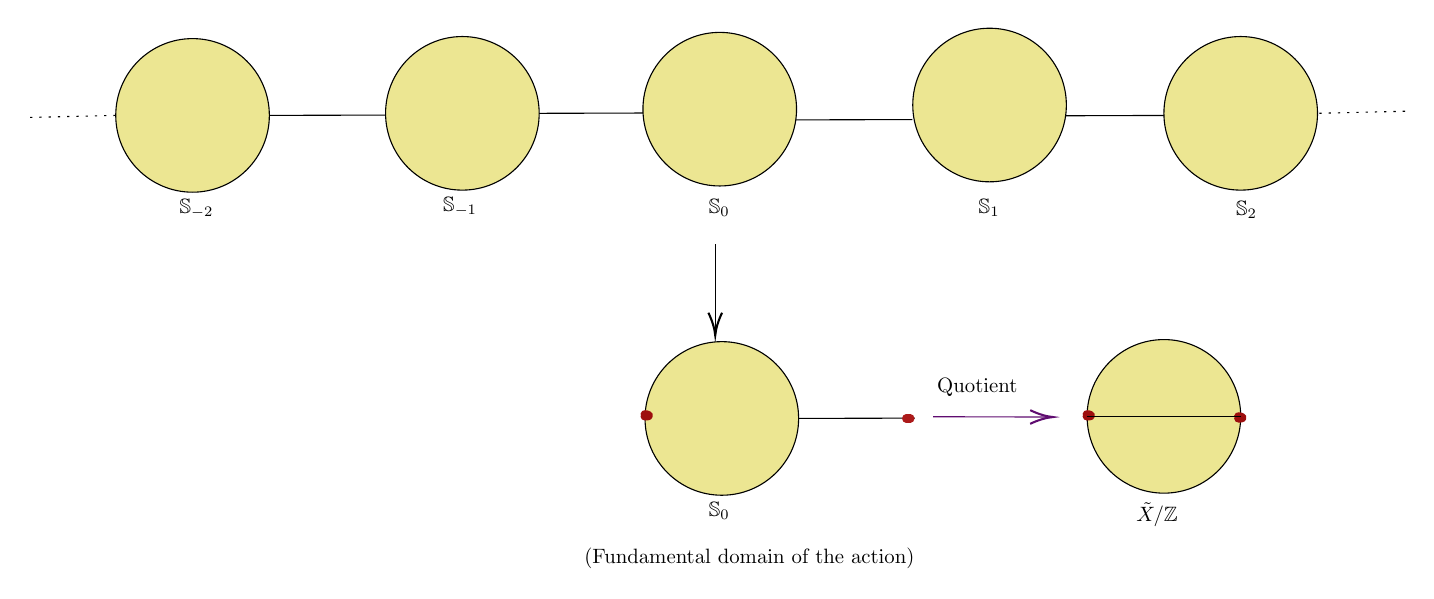
\begin{tikzpicture}[x=0.75pt,y=0.75pt,yscale=-1,xscale=1]
  %uncomment if require: \path (0,330); %set diagram left start at 0, and has height of 330
  
  %Shape: Circle [id:dp4026844205567903] 
  \draw  [color={rgb, 255:red, 0; green, 0; blue, 0 }  ,draw opacity=1 ][fill={rgb, 255:red, 236; green, 230; blue, 146 }  ,fill opacity=1 ] (12.17,44.83) .. controls (12.17,24.4) and (28.73,7.83) .. (49.17,7.83) .. controls (69.6,7.83) and (86.17,24.4) .. (86.17,44.83) .. controls (86.17,65.27) and (69.6,81.83) .. (49.17,81.83) .. controls (28.73,81.83) and (12.17,65.27) .. (12.17,44.83) -- cycle ;
  %Straight Lines [id:da6608283101748536] 
  \draw    (86.17,44.83) -- (142.17,44.67) ;
  %Shape: Circle [id:dp8634965486330941] 
  \draw  [color={rgb, 255:red, 0; green, 0; blue, 0 }  ,draw opacity=1 ][fill={rgb, 255:red, 236; green, 230; blue, 146 }  ,fill opacity=1 ] (142.17,43.83) .. controls (142.17,23.4) and (158.73,6.83) .. (179.17,6.83) .. controls (199.6,6.83) and (216.17,23.4) .. (216.17,43.83) .. controls (216.17,64.27) and (199.6,80.83) .. (179.17,80.83) .. controls (158.73,80.83) and (142.17,64.27) .. (142.17,43.83) -- cycle ;
  %Straight Lines [id:da24125011335625923] 
  \draw    (216.17,43.83) -- (272.17,43.67) ;
  %Shape: Circle [id:dp8486869396560328] 
  \draw  [color={rgb, 255:red, 0; green, 0; blue, 0 }  ,draw opacity=1 ][fill={rgb, 255:red, 236; green, 230; blue, 146 }  ,fill opacity=1 ] (266.17,41.83) .. controls (266.17,21.4) and (282.73,4.83) .. (303.17,4.83) .. controls (323.6,4.83) and (340.17,21.4) .. (340.17,41.83) .. controls (340.17,62.27) and (323.6,78.83) .. (303.17,78.83) .. controls (282.73,78.83) and (266.17,62.27) .. (266.17,41.83) -- cycle ;
  %Straight Lines [id:da698176486951738] 
  \draw    (340,47) -- (396,46.83) ;
  %Shape: Circle [id:dp5800447956821253] 
  \draw  [color={rgb, 255:red, 0; green, 0; blue, 0 }  ,draw opacity=1 ][fill={rgb, 255:red, 236; green, 230; blue, 146 }  ,fill opacity=1 ] (396.17,39.83) .. controls (396.17,19.4) and (412.73,2.83) .. (433.17,2.83) .. controls (453.6,2.83) and (470.17,19.4) .. (470.17,39.83) .. controls (470.17,60.27) and (453.6,76.83) .. (433.17,76.83) .. controls (412.73,76.83) and (396.17,60.27) .. (396.17,39.83) -- cycle ;
  %Straight Lines [id:da711655734243603] 
  \draw    (470,45) -- (500,44.91) -- (526,44.83) ;
  %Shape: Circle [id:dp8487288568740132] 
  \draw  [color={rgb, 255:red, 0; green, 0; blue, 0 }  ,draw opacity=1 ][fill={rgb, 255:red, 236; green, 230; blue, 146 }  ,fill opacity=1 ] (517.17,43.83) .. controls (517.17,23.4) and (533.73,6.83) .. (554.17,6.83) .. controls (574.6,6.83) and (591.17,23.4) .. (591.17,43.83) .. controls (591.17,64.27) and (574.6,80.83) .. (554.17,80.83) .. controls (533.73,80.83) and (517.17,64.27) .. (517.17,43.83) -- cycle ;
  %Straight Lines [id:da8241923062771945] 
  \draw  [dash pattern={on 0.84pt off 2.51pt}]  (12.17,44.83) -- (-30,45.83) ;
  %Straight Lines [id:da7621860142179304] 
  \draw  [dash pattern={on 0.84pt off 2.51pt}]  (633.33,42.83) -- (591.17,43.83) ;
  %Straight Lines [id:da5654821669824697] 
  \draw    (301,107) -- (301,148.83) ;
  \draw [shift={(301,150.83)}, rotate = 270] [color={rgb, 255:red, 0; green, 0; blue, 0 }  ][line width=0.75]    (10.93,-3.29) .. controls (6.95,-1.4) and (3.31,-0.3) .. (0,0) .. controls (3.31,0.3) and (6.95,1.4) .. (10.93,3.29)   ;
  %Shape: Circle [id:dp21056323721972636] 
  \draw  [color={rgb, 255:red, 0; green, 0; blue, 0 }  ,draw opacity=1 ][fill={rgb, 255:red, 236; green, 230; blue, 146 }  ,fill opacity=1 ] (267.17,190.83) .. controls (267.17,170.4) and (283.73,153.83) .. (304.17,153.83) .. controls (324.6,153.83) and (341.17,170.4) .. (341.17,190.83) .. controls (341.17,211.27) and (324.6,227.83) .. (304.17,227.83) .. controls (283.73,227.83) and (267.17,211.27) .. (267.17,190.83) -- cycle ;
  %Straight Lines [id:da8717605813156255] 
  \draw    (341.17,190.83) -- (397.17,190.67) ;
  %Shape: Free Drawing [id:dp0266335380840097] 
  \draw  [color={rgb, 255:red, 157; green, 14; blue, 14 }  ,draw opacity=1 ][line width=3] [line join = round][line cap = round] (267,188.83) .. controls (268.35,188.83) and (270.8,189.83) .. (267,189.83) ;
  %Shape: Free Drawing [id:dp05418555348732901] 
  \draw  [color={rgb, 255:red, 172; green, 26; blue, 26 }  ,draw opacity=1 ][line width=3] [line join = round][line cap = round] (393,190.83) .. controls (395.67,190.83) and (395.67,190.83) .. (393,190.83) ;
  %Shape: Circle [id:dp2818577737183854] 
  \draw  [color={rgb, 255:red, 0; green, 0; blue, 0 }  ,draw opacity=1 ][fill={rgb, 255:red, 236; green, 230; blue, 146 }  ,fill opacity=1 ] (480.17,189.83) .. controls (480.17,169.4) and (496.73,152.83) .. (517.17,152.83) .. controls (537.6,152.83) and (554.17,169.4) .. (554.17,189.83) .. controls (554.17,210.27) and (537.6,226.83) .. (517.17,226.83) .. controls (496.73,226.83) and (480.17,210.27) .. (480.17,189.83) -- cycle ;
  %Straight Lines [id:da14300264469322888] 
  \draw [color={rgb, 255:red, 95; green, 12; blue, 112 }  ,draw opacity=1 ]   (406,190) -- (461.67,190.16) ;
  \draw [shift={(463.67,190.17)}, rotate = 180.17] [color={rgb, 255:red, 95; green, 12; blue, 112 }  ,draw opacity=1 ][line width=0.75]    (10.93,-3.29) .. controls (6.95,-1.4) and (3.31,-0.3) .. (0,0) .. controls (3.31,0.3) and (6.95,1.4) .. (10.93,3.29)   ;
  %Shape: Free Drawing [id:dp7791710762992532] 
  \draw  [color={rgb, 255:red, 157; green, 14; blue, 14 }  ,draw opacity=1 ][line width=3] [line join = round][line cap = round] (480,188.83) .. controls (481.35,188.83) and (483.8,189.83) .. (480,189.83) ;
  %Shape: Free Drawing [id:dp39512041048805213] 
  \draw  [color={rgb, 255:red, 157; green, 14; blue, 14 }  ,draw opacity=1 ][line width=3] [line join = round][line cap = round] (553,189.83) .. controls (554.35,189.83) and (556.8,190.83) .. (553,190.83) ;
  %Straight Lines [id:da5180415087093939] 
  \draw    (480.17,189.83) -- (554.17,189.83) ;

% Text Node
\draw (297,83.4) node [anchor=north west][inner sep=0.75pt]  [xscale=0.75,yscale=0.75]  {};
% Text Node
\draw (297,84.4) node [anchor=north west][inner sep=0.75pt]  [xscale=0.75,yscale=0.75]  {$\s_0$};
% Text Node
\draw (427,84.4) node [anchor=north west][inner sep=0.75pt]  [xscale=0.75,yscale=0.75]  {$\s_1$};
% Text Node
\draw (551,85.4) node [anchor=north west][inner sep=0.75pt]  [xscale=0.75,yscale=0.75]  {$\s_2$};
% Text Node
\draw (169,83.4) node [anchor=north west][inner sep=0.75pt]  [xscale=0.75,yscale=0.75]  {$\s_{-1}$};
% Text Node
\draw (42,84.4) node [anchor=north west][inner sep=0.75pt]  [xscale=0.75,yscale=0.75]  {$\s_{-2}$};
% Text Node
\draw (297,230.4) node [anchor=north west][inner sep=0.75pt]  [xscale=0.75,yscale=0.75]  {$\s_0$};
% Text Node
\draw (503,230.4) node [anchor=north west][inner sep=0.75pt]  [xscale=0.75,yscale=0.75]  {$\tilde{X}/\Z$};
% Text Node
\draw (407,170.4) node [anchor=north west][inner sep=0.75pt]  [xscale=0.75,yscale=0.75]  {$\text{Quotient}$};
%Textnode
\draw (120,121) node  [xscale=0.75,yscale=0.75] [align=left] {\begin{minipage}[lt]{68pt}\setlength\topsep{0pt}

\end{minipage}};
% Text Node
\draw (237,252.4) node [anchor=north west][inner sep=0.75pt]  [xscale=0.75,yscale=0.75]  {$\text{(Fundamental domain of the action)}$};


\end{tikzpicture}
\caption{Description of $\tilde{X}$}
\end{figure}
\noindent As in the above picture, we have aligned $\tilde{X}$ along $X$-axis. Now we \textbf{claim} $\s_0 \cup L_0$ is the fundamental domain of this action. Any point in $\tilde{X}$ must lie in a sphere $\s_n$ or in a line $L_m$, by acting $-n$ or $-m$ respectively to this point we will get a point in $\s_0$ or $L_0$ respectively. Thus, $\s_0\cup L_0$ is fundamental domain of this action. Note that, $1.(0,0,-1) = (0,0,2)$, which means end point of $L_0$ and one pole of $\s_0$ are identified in the orbit space $\tilde{X}/\Z$ (as shown in the above figure with \textcolor{red}{red} mark). So, the orbit space $\tilde{X}/\Z$ is exactly the space, $$X := \qty{\text{ A sphere } \s^2 \text{ along with the diameter joining noth-pole and south-pole }}$$
From the above discussion we can conclude that, $\pi : \tilde{X} \to \tilde{X}/\Z \simeq X$ is a covering space. We are yet to show $\tilde{X}$ is \textbf{simply connected}. It is enough to prove the finite collection $\tilde{X}_k := \bigcup_{n \in [-k,k]} (\s_n\cup L_n)$ is simplicity connected, i.e. $\pi_1(\tilde{X}_k) = \qty{0}$. Now by taking $\operatorname{colim} \tilde{X}_k$, we will get $\tilde{X}$ and thus $\pi_1(\tilde{X})=\qty{0}$. By inductive argument it boils down to proving $\s_0 \cup L_0 \cup \s_1$ is simply connected. Take the open covers $U = \s_0 \cup \qty{(0,0,t) :t \in [1,1+\epsilon)}$ and $V = \s_1 \cup \qty{(0,0,t) : t \in (1+\frac{\epsilon}{2},2]}$. Note that, $U\cap V$ is an open interval $\qty{(0,0,t): t \in (1+\frac{\epsilon}{2},1+\epsilon)}$, which is simply connected. Also, both $U$ and  $V$ has deformation retract onto the $2$-sphere $\s^2$, which have trivial fundamental group. By \textbf{\textsf{SVK}} we can say the above space is simply connected. Hence, $\tilde{X}$ is simply connected and $\pi : \tilde{X} \to \tilde{X}/\Z \simeq X$ is the universal covering. By the \textbf{\textsf{classification of covering space}}, we can say, $\pi_1(X) = \Z$.


 \section{Problem 7}
 \begin{prob}{}
    The Borsuk-Ulam theorem states that if $f : \s^n \to \R^n$ is continuous, then there exists $x \in \s^n$ such that $f(x) = f(-x)$. Prove the Borsuk-Ulam theorem for $n=1,2$. 
 \end{prob}
 \sol For $n=1$ if there exists a map $f : \s^1 \to \R^1$ such that, $f(x) \neq f(-x)$ for all $x\in \s^1$. Consider the map $g(x) = \frac{f(x)-f(-x)}{\abs{f(x)-f(-x)}}$. It is clearly a continuous map $g : \s^1 \to \s^0=\qty{-1,1}$. If for some $x$, $g(x)$ is $+1$ then for $-x$ it takes the value $-1$. We know continuous map preserves connectedness. $\s^1$ is connected but $\s^0$ is not. So, $g(\s^1)$ has to lie in one of the connected components, but it is not possible by the above observation. So, there must exist a point $x \in \s^1$ such that, $f(x)=f(-x)$. 
 

 \vspace*{0.2cm}

 \begin{wrapfigure}{r}{5cm}
    \begin{tikzcd}
        {\s^2} && {\s^1} \\
\\
{\R P^2} && {\R P^1 = \s^1}
\arrow["{p_2}"', from=1-1, to=3-1]
\arrow["{p_1}", color={rgb,255:red,214;green,92;blue,92}, from=1-3, to=3-3]
\arrow["g", from=1-1, to=1-3]
\arrow["{\bar{g}}"', color={rgb,255:red,214;green,92;blue,92}, from=3-1, to=3-3]
\arrow["{\tilde{g}}", color={rgb,255:red,214;green,92;blue,92}, dotted, from=3-1, to=1-3]
    \end{tikzcd}
\end{wrapfigure}


\noindent Again for contradiction let's assume there is a continuous map $f:\s^2 \to \R^2$ such that, $f(x)\neq f(-x)$ for all $x \in \s^2$. Consider, $g(x) = \frac{f(x)-f(-x)}{\norm{f(x)-f(-x)}}$. This is by definition a continuous map from $\s^2 \to \s^1$. Let, $p_i : \s^i \to \R P^i$ be the quotient maps that takes a piar of antipodal points to ta point. We know these maps are covering map (done in class). Note that, $g(x) = - g(-x)$, i.e. it takes a pair of antipodal point to a pair of antipodal point. So it will induce a map $\bar{g} : \R P^2 \to \R P^1$.

\vspace*{0.2cm}

\noindent We know, $\pi_1(\R P^2)$ is $\Z/2\Z$ and $\pi_1(\R P^1)=\Z$. The induced homomorphism $\tilde{g}_* : \pi(\R P^2) \to \pi_1(\R P^1)$ must be a trivial homomorphism as the fundamental group of $\R P^2$ is finite. Thus can extend the map $\bar{g}$ to a map $\tilde{g} : \R P^2 \to \s^1$ such that the red triangle in the above diagram commutes i.e. $p_1 \circ \tilde{g} = \bar{g}$. From the commutativity of the square we can say $p_1^{-1}\circ \bar{g} \circ p_2(s)$ can take values either $g(s)$ or $g(-s)$. Which means, $\tilde{g} \circ p_2(s)= \tilde{g} \circ p_2(-s)$ can take two one of the values $g(s)$ or $g(-s)$. In either case we can get a $t$ (it is $s$ or $-s$) such that, $\tilde{g} \circ p_2(t) = g(t)$. By the fundamental theorem of covering space theory we can say $\tilde{g} \circ p_2 = g$ for all $t \in \s^2$. But it is not possible as $g(t) = - g(-t)$ and $\tilde{g} \circ p_2(t) = \tilde{g} \circ p_2 (-t)$.  So there is a point $x \in \s^2$ such that, $f(x)=f(-x)$. $\hfill \blacksquare$
------------------------------------------------------------------------------------------------------------------------------------------------

\noindent \textbf{\textsf{Remark:}} We can prove the `Borsuk-Ulam theorem' for higher $n$ in the same way. But in order to showing the extension $\tilde{g}$ exist, we need to deal with `Hurewicz isomorphism' and cohomology ring of $\R P^2$ with the coefficients in $\Z/2\Z$.


\section{Problem 8}

\begin{prob}{}{}
    Prove that there is a double covering of the Klein bottle by the torus. Take the definition of the Klein bottle as $[0,1] \times [0,1]/\sim$ where $\sim$ is the equivalence relation generated by $(x,0) \sim (x,1)$ and $(0,1-y) \sim (1,y)$.
\end{prob}

\sol For the simplicity of notation, let's call $K$ be the Klein bottle and $T$ be the one-holed torus. We know from \textbf{Problem 2}, $\pi_1(K) = \inp{a}{b : aba^{-1}b = 1}$. Now consider the action of homeomorphisms $\varphi_1,\varphi_2$ on $\R^2$ defined as, $(x,y)\mapsto (x+1,y)$ and $(x,y)\mapsto (-x,y+1)$ respectively. Let,$G$ be the group generated by these homomorphisms under composition. Note that, $\varphi_2\circ \varphi_1 = \varphi_1^{-1} \circ \varphi_2$. So, $G = \inp{\varphi_1}{\varphi_2 : \varphi_2\circ \varphi_1 = \varphi_1^{-1} \circ \varphi_2}$ is the group generated by the homomorphisms. It is not hard to notice that, $G = \pi_1(K)$. We are basically looking at the action of $G \curvearrowright \R^2$. Note that,
\begin{align*}
    \varphi_2 \circ \varphi_1 \circ \varphi_2 (x,y) &= (x-1,y+2)\\
    &= \varphi_1^{-1} \circ \varphi_2^2(x,y)\\
    \varphi_1 \circ \varphi_2 \circ \varphi_1 &= (-x,y+1) \\
    &= \varphi_2
\end{align*}
So any element in the group $G$ can be written as $\varphi_1^m \circ \varphi_2^n$ for some $m,n\in \mathbb{Z}$. Generators of the group are distance preserving homeomorphisms. So and element of the group is distance preserving homeomorphism. For any point $(x,y) \in \R^2$ take an open disk centred at that point with diameter $d< 1$. Call this disk $D_{(x,y)}$, we will show, $g(D_{(x,y)}) \cap h(D_{(x,y)}) = \emptyset$. Which means the group action is properly discontinuous. 
Let, $g$ is an element in $G$ then $g = \varphi_1^{m}\circ \varphi_2^{n}$. So, $g.D_{(x,y)} = \{((-1)^n +u+m,v+n) : (u,v) \in D_{(x,y)}\}$. If there is a point $(x',y')$ the intersection of $D_{(x,y)}$ and $g.D_{(x,y)}$ then distance between $(x',y')$ and $((-1)^nx'+m,y'+n)$ is $< d$. 
$$\sqrt{(((-1)^n-1)x'+m)^2+ n^2} \le d <1$$
since $n$ is an integer we must have $n =0$ and then $m^2 \le d<1$ which means $m=0$ i.e $g = e$. If $g$ is not identity then $g(D_{(x,y)}) \cap (D_{(x,y)}) = \emptyset$. We can see that $\varphi_1(x,y),\varphi_2(x,y)$ are at-least $1$-unit distance apart from $(x,y)$. By the similar calculation as above, for any two distinct element $g,h \in G$ we can say that $g(x,y)$ and $h(x,y)$ are at-least $1$-unit apart from each other.  

\vspace*{0.2cm}

\noindent If $(x, y)$ lies in $\mathbb{R}^2$, by applying the homeomorphism $\varphi_1^m$ for some appropriate integer $m$ to $(x, y)$, we can convert it to a point $(a, y)$ where $a \in[0,1)$ (this is like taking fractinal part). Then by applying the homeomorphism $\varphi_2^n$ for some appropriate integer $v$ to $(a, y)$, we get the point $\left((-1)^n a, b\right)$ where $b \in[0,1]$. If $v$ is even, we get a point lying in $[0,1]^2$ lying in the same equivalence class as $(x, y)$ in $\mathbb{R}^2 / G$. Otherwise another application of $g$ gives us such a point lying in $[0,1)^2$. Moreover no two points in $[0,1]^2$ lie in the same equivalence class of $\mathbb{R}^2 / G$. So $\mathbb{R}^2 / G$ can be identified with the space $[0,1]^2$ with the quotient topology induced as it is the fundamental domain for the action. 

\vspace*{0.2cm}

\noindent Consider the unit square $\mathcal{S} = [0,1]\times [0,1]$ We can see that any orbit of the given action has a representative on $\mathcal{S}$. If we look at the point interior of the square, they are representative of themself. This is because any $g \in G$ must take a point atleast $1$-distance apart from itself by translation. We will look on the boundary of the square where, the points of the form $(0,y)$ are representative with $(1,y)$ (by $\varphi_1$) and the points of the form $(x,1)$ representative with $(1-x,0)$ (by $\varphi_1 \circ \varphi_2^{-1}$). We can also see all four vertex belong to same orbit. $(0,y)$ and $(x,1)$ can't be representative to eachother if $0<x,y<1$ this is clearly because the distance in $y$-coordinate is greater than $0$ but less than $1$. Similarly we can show $(0,y)$,$(1,y)$ can't be representative with $(x,0)$ and $(x,1)$ in any means. From the given identification we can see the orbit space $\R^2 /G$ is Klein bottle $K$. 

\vspace*{0.2cm}

\noindent Now we will show \textbf{$G = \pi_1(K)$ contains a copy of $\Z \oplus \Z$} and it's index as a subgroup of $G = \pi_1(K)$ is $2$. Recall the representation of the group,(where $\varphi_2 =a,\varphi_1=b$) $$G=\pi_1(K) = \inp{a}{b : aba^{-1}b = 1}$$
Take the subgroup $H$ generated by, $a^2,b$. Notice that, \begin{align*}
    a^2b & = a(ab) \\
    &= ab^{-1}a \\
    &= ab^{-1}a^{-1}a^2 \\
    &= (aba^{-1})^{-1}a^2\\
    &= b^2a
\end{align*}
So, $H \cong \Z \oplus \Z$ and \textbf{index of this group is $2$} as we are quotienting out $G$ with $\inp{a^2}{b}$. Now we will restrict the action $G \curvearrowright \R^2$ to $H$ any element of $H$ must look like $h=\varphi^{n} \circ \varphi^{2m}$, where $m,n \in \Z$. Any point $(x,y)$ will go to $h.(x,y) = (x+n,y+2m)$ by the action of $h \in H$. In this case we can notice the fundamental domain is $[0,1]\times [-1,1]$. The identification hold here is, $(x,1)\sim (x,-1)$ and $(0,y)\sim (1,y)$. So the orbit-space $\R^2 / H$ is torus $T$. By the \textbf{\textsf{classification theorem of covering spaces}}, we can say, there is a $2$-sheeted covering $p:T \to K$. 



\end{document}

